\documentclass[acmsmall]{acmart}

\usepackage{caption}
\usepackage{subcaption}
\usepackage{cleveref}
\usepackage{appendix}

\captionsetup[subfigure]{subrefformat=simple,labelformat=simple}
\renewcommand\thesubfigure{(\alph{subfigure})}


\begin{document}
\title{Denoising Shadows Using Image-to-Image Translation Networks}

\author{Daniel Gerzhoy}
\author{Justin Shen}
\maketitle

\section{Introduction}
\label{sec:intro}

This work reports the work done and results achieved for the final project in CMSC740: Advanced Computer Graphics. We were tasked with using image-to-image translation deep learning networks to add rendering effects, specifically creating low-noise shadows from images rendered with noisy shadows from area lights.

\section{Background}
\label{sec:background}

\subsection{Area Lights and Shadows}

\begin{figure}
	\Description[<short description>]{<long description>}
	\centering
	\subcaptionbox{1 Sample per pixel\label{sf:lowRes}}%
		[0.25\textwidth]{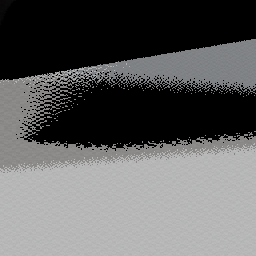
\includegraphics[width=.25\textwidth]{images/lowresshadow.png}}
	\hspace{.05\textwidth}
	\subcaptionbox{16 Samples per pixel\label{sf:hiRes}}%
		[0.25\textwidth]{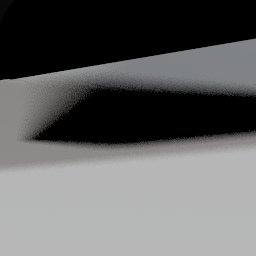
\includegraphics[width=.25\textwidth]{images/highresshadow.png}}
	\caption{Scene rendered with very few samples per pixel vs same scene rendered with more samples. The scene has two lights creating 2 distinct and overlapping shadows. Notice the edges of the shadows are very noisy in the first case}	
	\label{f:ShadowNoise}
\end{figure}

The source of the noisy shadows we seek to denoise is Monte-Carlo rendering. When a ray is drawn from the camera origin and it hits an object in scene, a light is sampled, and a shadow ray is drawn between the hit point and a sampled point on the light. If that ray hits anything in the scene the radiance from the light source does not reach the camera, creating a shadow. For one sample, one hit point is found and one light is sampled X times. If X is low and the light is large, or if the global sample rate is low a hit point might erroneously be cast in shadow because the randomly sampled light point it found was occluded, even if there are points on the lights in view of this hit point. This happens most often closer to the smooth edges of the shadows. Figure \ref{f:ShadowNoise} shows a scene with 2 lights and an object casting 2 overlapping shadows. In fig \ref{sf:lowRes} near the edges of the shadows, there are not enough shadow rays to create smooth shadows, the gradient is very noisy.

\subsection{Original Network}

In order to denoise shadows in a given rendered scene, we make use of the image-to-image translation network to train a conditional adversarial network to perform the denoising. The network eliminates the need hand-engineer mapping and loss function and has shown success in other tasks such as synthesizing photos from label maps, reconstructing objects from edge maps, and colorizing images \cite{DBLP:journals/corr/IsolaZZE16}. The network consists of a generator $G$ based on an encoder-decoder architecture with skip connection (like a ``U-Net") and a discriminator $D$, call \textit{Patch} GAN, to convolutionally classify each $N \times N$ patch of the image as real or fake. The objective of this conditional GAN  is \begin{equation}
    \mathcal{L}_{cGAN}(G,D) = \mathbb{E}_{x,y}[\log{D(x,y)}] + \mathbb{E}_{x,z}[\log{(1 - D(x,G(x,z)))]}
\end{equation} 
where $G$ tries to minimize this objective against $D$ that tries to maximize it. The conditional GAN loss is mixed with the L1 loss $\mathcal{L}_{L1}(G) = \mathbb{E}_{x,y,z} [ \| y - G(x,z) \|_1]$ to yield the final objective for the network: \begin{equation}
    G* = \arg \min_G \max_D \mathcal{L}_{cGAN}(G,D) + \lambda \mathcal{L}_{L1}(G)
\end{equation}

Using this network we made use of different training input pairs and minor architecture tweaks to work toward our goal.

\section{Data Generation}
\label{sec:datagen}

\subsection{Initial Scenes}
\label{subsec:initScenes}

We began collecting scenes to generate data by looking at the pbrt-v3-scenes repository~\cite{scenes}. We chose a few simple scenes containing area lights to begin with, to extract multiple data points from one scene quickly and automatically, we created a script that would rotate (rotate.py) the lights in the scene around an axis. The intuition for this was that with lights coming at the object from different positions, the network would learn different shadows can come from the same shape.

\subsection{Scene Generator}
\label{subsec:sceneGen}

However it became clear that using real scenes to generate data would take too much time even with automatic light rotation, due to the custom nature of each of the scenes. We then began to experiment with automatically generated scenes by a script (sceneGenerator.py). The basic idea was to create a scene with a floor and insert randomly generated shapes (spheres or cubes) above that floor in random locations, and randomly generated area lights (spherical) above the shapes.

With the location of the floor fixed, the shapes were placed in placed on a 3D grid above the floor (the shape slab) with no shapes occupying the same place. The size of each shape is randomly chosen from a set of sizes chosen so that no shapes overlap, or overlap only a little such that a shape cannot contain the entirety of another shape. Above the plane of the shapes, the area lights are placed similarly on a 3D grid (the light slab). The grid places the shapes and lights at different angles to each other and the floor, creating different shadows each time, in different locations relative to the shapes, and possibly overlapping.

The number of shapes and lights desired is provided as an input to the script, as well as the number of arrangements of shapes and of lights. A significant feature of the scene generator is that every configuration of shapes in the shape slab, is combined with all different configuration of the lights in the light slab. The hope is that seeing the same shape configuration with different shadows, again teaches the network that different shadows come from different shapes.

As we trained and tested the network with the generated scenes (to be discussed in more detail in Section\ref{sec:train} ) we discovered that it was not preserving the original colors and textures of the test scene, so we added random colors and textures to the shapes and floor, hoping that this would teach the network that differently colored and textured shapes create the shadows. We created complex textures by mixing random textures hierarchically. At the bottom level a texture was solid, checkerboard, or polka dots. Those are combined with scaling (multiplication of pixel values for 2 textures), linear interpolation between two textures, checkers, or polka dots.

Finally the scenes could be rotated so that rather than light coming from above and shining down onto a floor, shadows could be cast from area lights behind the camera onto a wall. 

\begin{figure}
	\Description[<short description>]{<long description>}
	\centering
	\subcaptionbox{A vertical view image with complex textures and shapes\label{sf:vert}}%
		[0.25\textwidth]{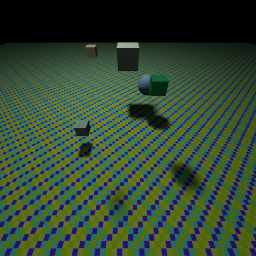
\includegraphics[width=.25\textwidth]{images/gen1.png}}
	\hspace{.05\textwidth}
	\subcaptionbox{A horizontal view image with complex textures and shapes\label{sf:horiz}}%
		[0.25\textwidth]{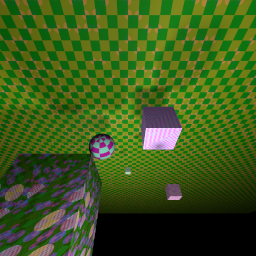
\includegraphics[width=.25\textwidth]{images/gen2.png}}
	\hspace{.05\textwidth}
	\subcaptionbox{Depth Map for vertical view\label{sf:depth}}%
		[0.25\textwidth]{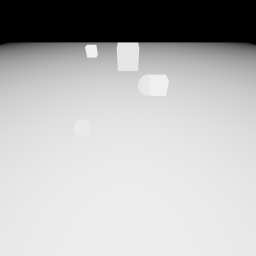
\includegraphics[width=.25\textwidth]{images/gen1_depth.png}}
	\caption{Generated Scenes}	
	\label{f:exampleScenes}
\end{figure}

Figure \ref{sf:vert} and \ref{sf:horiz} show examples of automatically generated scenes with complex textures.

\subsection{Depth Map Generation}
\label{subsec:depthMap}

Creating the depth map was a simple alteration to PBRT. We added a new integrator that before rendering begins calculates from the camera what the maximum distance to any point in the scene is. This is acheived not by checking every vertex in the scene, but by using the points of the bounding volume. The maximum distance is the distance to the furthest point of the bounding volume. Then during renduring -- given a ray, the integrator finds where it intersects the scene and how far along the ray it does so. It then outputs a gray scale value equal to the distance found divided by the max distance. The depth map for \ref{sf:vert} is shown in \ref{sf:depth}. Note that if the depth is found to be infinite (the ray does not intersect the scene) black radiance is returned.

\section{Training}
\label{sec:train}

To train the network to learn how to denoise shadow in a given noisy input, we experimented with training the original image to image translation network with different generated dataset and different number of training epoch. %The purpose of experimenting with different datasets was to test whether we are able to generate scenes that can generally capture the shadowing effects in any given scene beyond our generated scene. Meanwhile, changing the number of training epoch attempts to 
To perform the network training we make use of a version of the network implemented in Tensorflow found at \url{https://github.com/affinelayer/pix2pix-tensorflow}

We also attempt to denoise shadow by extending the network to take in depth map information as an additional input. This is done simply by reshaping the convolutional layers to take in depth map as a fourth channel of the input image pair.  Given an input with depth map (represented as a $256\times256\times4$ tensor), the network outputs the denoise image in the also in the form of a $256\times256\times4$ where the last layer of the output can be removed to yield the typical RGB image output as the usual $256\times256\times3$ tensor.


\section{Results}
\label{sec:results}

\subsection{Preliminary Scenes Results}
\label{subsec:prelim_scenes}

We first train the network using a dataset of images rendered from the book scenes as described in Section\ref{subsec:initScenes} and then test the network with some of the withheld data. The preliminary result seen below serve to establish the level of denoising we want to be able to achieve from training the original network or the modified network with an autogenerated dataset. The idea is that the shadow generation model for autogenerated scenes should come close the shadow generation model for the book scene and other more complex scenes.

\begin{figure}[ht!]
	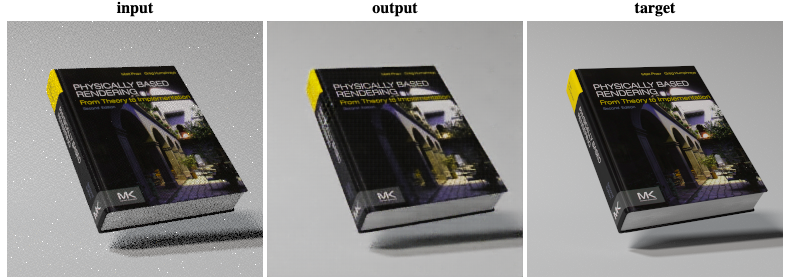
\includegraphics[width=\textwidth]{images/preliminary.png}
	\label{f:prelim}
	\caption{Input and output images from the network trained with initial sample scene as data, as well as the expected target image.}
\end{figure}

\subsection{Autogenerated Scenes Results}
\label{subsec:auto_scenes}

As the project progress we made progressive change to the automatic scene generator in an attempt to more fully capture the general shadow generation model. The initial scenes generated do not include any color variation while the next iteration do vary the color (as well as shape). The visual results of training the network with images rendered from those generated scenes are detailed in Section\ref{subsubsec:no_texture} and Section\ref{subsubsec:with_color} below. The automatically generated scenes used are both are composed of a combination of scenes with 2, 3, or 5 objects (4 arrangement for each) with 1, 2, or 4 light sources (10 arrangement for each), for a total of 360 image pairs for training. The number of training epoch is 200 for both. \newpage

\subsubsection{Scenes without Color Variation}
\label{subsubsec:no_texture}

Below is the result from the network trained with images with no color or shape variation tested on some rendered images from the book scene. The network seems unable to learn color variation.

\begin{figure}[ht!]
	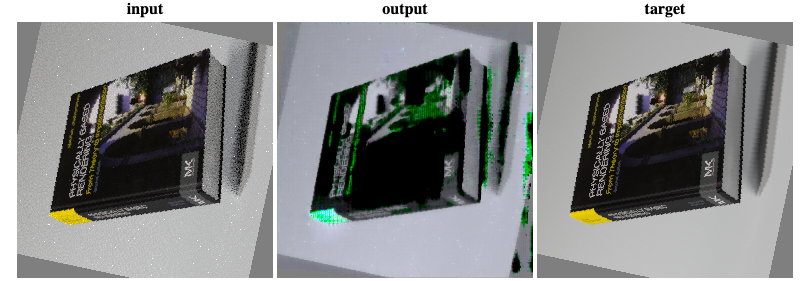
\includegraphics[width=\textwidth]{images/experiment1.png}
	\label{f:exp1}
	\caption{Input and output images from the network trained with images rendered from autogenerated scenes with only green spherical objects, along with the expected target image. Note that at this point in the project random rotation is incorporated in generating the dataset but is removed in later iteration of the training process.}
\end{figure}

\subsubsection{Scenes with Color Variation}
\label{subsubsec:with_color}

Below is the result from the network trained with images with both color and shape variation tested on rendered images from the book scene and some autogenerated scenes.

\begin{figure}[ht!]
	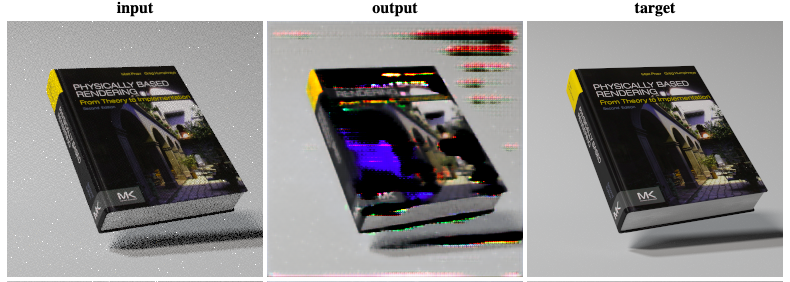
\includegraphics[width=\textwidth]{images/experiment2.png}
	\label{f:exp2}
		\caption{Input and output images of testing book scenes from the network trained with images rendered from autogenerated scenes with color and shape variation, along with the expected target image.}
\end{figure}

\begin{figure}[ht!]
	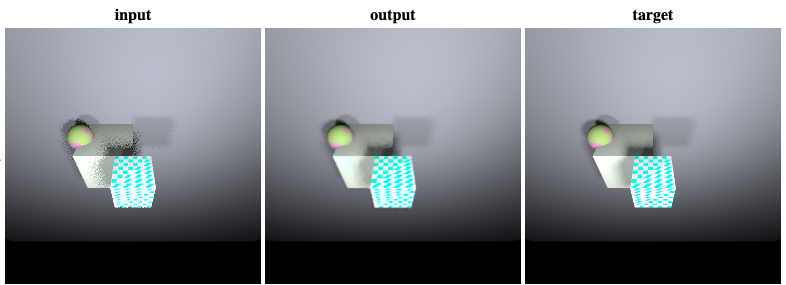
\includegraphics[width=\textwidth]{images/experiment3.png}
	\label{f:exp3}
		\caption{Input and output images of testing autogenerated scenes from the network trained with images rendered from autogenerated scenes with color and shape variation, along with the expected target image.}
\end{figure}

\subsubsection{Scenes with Color and Texture Variation}
\label{subsubsec:with_texture}

In addition to the  360 image pairs from before, we add an additional set of images rendered with the scene renderer in Section\ref{subsec:sceneGen} which now includes full texture, color, and shape variation in the autogenerated scenes. The newly added scenes includes scenes with 1, 4, or 6 objects at 5 different arrangements, and each scene is rendered with either 2, 3, or 5 different lights each arranged in 9 different ways. This results in an additional 405 training images. Below is the result from the network trained with images with both color, texture, and shape variation tested on rendered images from the book scene as just described. The coloring of the book scene is much better preserved compared to that from the network trained with images from scenes with only color and shape variation.

\begin{figure}[ht!]
	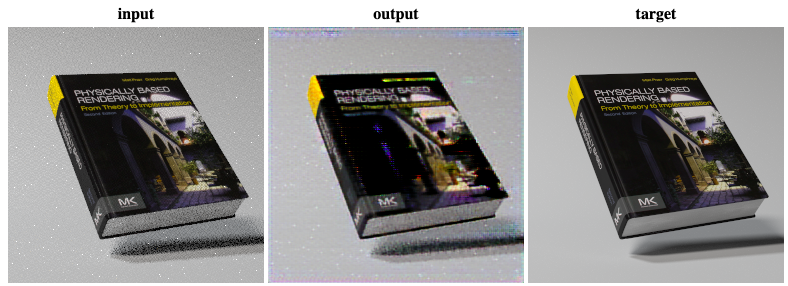
\includegraphics[width=\textwidth]{images/experiment4.png}
	\label{f:exp4}
		\caption{Input and output images of testing book scenes from the network trained with images rendered from autogenerated scenes with color, texture, and shape variation, along with the expected target image.}
\end{figure}

%\begin{figure}[ht!]
%	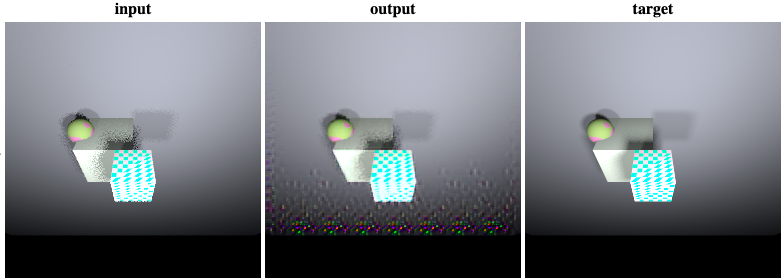
\includegraphics[width=\textwidth]{images/experiment5.png}
%	\label{f:exp5}
%		\caption{Input and output images of testing autogenerated scenes from the network trained with images rendered from autogenerated scenes with color, texture and shape variation, along with the expected target image.}
%\end{figure}

\newpage

\subsection{Results with Depth Map}
\label{subsec:depth}

Result incorporating depth map into the network in comparison to the same input without depth map information is included below. Both training are done with 200 epoch and with the data set described in Section\ref{subsubsec:with_texture}. Perceptually there is not much difference incorporating the depthmap into the training.

\begin{figure}[ht!]
	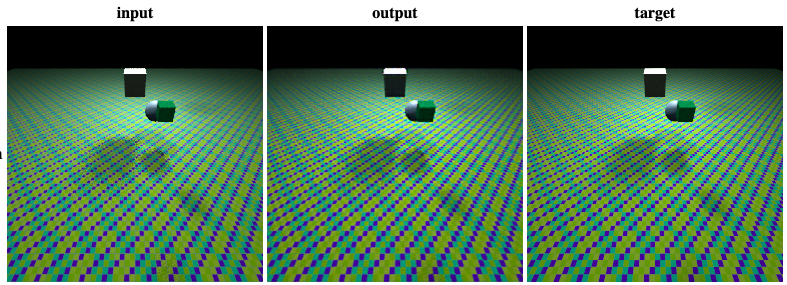
\includegraphics[width=\textwidth]{images/with-depth.png}
	\label{figDepth}
		\caption{Input and output images of autogenerated scene from the network trained with images rendered from autogenerated scenes with color, texture, shape variation, and depth information, along with the expected target image.}
\end{figure}

\begin{figure}[ht!]
	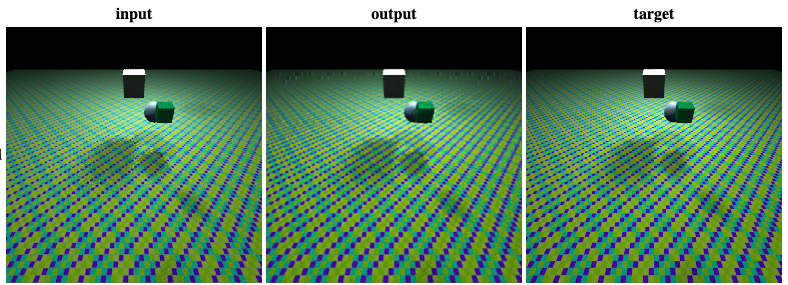
\includegraphics[width=\textwidth]{images/no-depth.png}
	\label{noDepth}
		\caption{Result from the network with the same input from Figure\ref{figDepth} but without depth map input}
\end{figure}

\newpage
%v2 shows result of testing with the book scene, the result here captures the color book the much better than before the random color and textures are added so the new addition definitely did help a lot. It is still not quite perfect though. I believe the network still does not quite know how to deal with preserving the background and aesthetic of the scene. To address this I think it would be good to change up the color of the background. Also, your suggestion of increasing the maximum size sounds good to me.

%v3 shows the result of testing with the generated scene. The result is much better as expected since we are evaluating the network with data similar to the training data. This suggests to me that either the network is overfitting or the autogenerated scenes are not generalizable to more complex scenes (as in the case of book scene above). To that end, I am running a few more test experimenting with the maximum number of training epoch to test this idea out. I will also run training with both the autogenerated scene and a more complex scene to see if that improves generalizability as well.




\section{Future Work}
\label{sec:future}

Two possible pathway for future work could come in the areas of additional data provided by the renderer for each scene or automatic scene generation for more training data.

Additional data could come in the form of information about where the lights lie relative to the rest of the scene, or else voxel grids describing the entire scene and not just a depth map of the objects casting shadows. This would provide the network with information about where the shadows should be cast, perhaps improving the color and texture properties of the resultant images.

Generating more complex scenes in random patterns with the generator could help generalize the things learned from automatically generated scene to more complex scenes. If many more smaller shapes were to be generated in each generated scene, analogous to the pieces of a Riemann sum, the final result would be a more realistic understanding of how shapes cast shadows.

\section{Conclusion}
\label{sec:conclusion}

We have experimented with Denoising Shadows using an Image-to-Image translation network, trained with automatically generated data. We began with simple generated scenes, that did not provide enough variation in color, or texture to generalize to real more complex scenes. We then added these features and observed improvements to color retention. While the network is able to successfully denoise shadow from the autogenerated scenes, more work remains to achieve the same level of denoising in the more complex scenes.

We added a depth map channel to the network and observed minimal improvement to the final output of the network in terms of shadow denoising. The extension to the network to incorportate the depth information was done as an additional channel and minor changes to the convolutional layer's shape. More complex modification could be done in the future as well to better utilize depth information for shadow denoising. 

\appendix
\appendixpage
Our changes to the PBRT render, Image-to-Image network, and scene generator can be found in the following git repository:
\begin{itemize}
    \item \url{https://github.com/dgerzhoy/pbrt-v3-CMSC740-dgerzhoy.git}
    \item \url{https://github.com/jstnshen/pix2pix-tensorflow.git}
\end{itemize}

\section{Depth Map Renderer}

The integrator created in the renderer is contained in depthmap.h and depthmap.cpp in /pbrt-v3/src/integrators

\section{Scene Generator and Rotator}

The scene generator is located at pbrt-v3/generator/sceneGenerator/sceneGenerator.py
\linebreak The rotator script is located at /pbrt-v3/rotator/rotate.py

\section{Depth Map Image-to-Image Translation Network}

The modified network is contained in shadow2pix.py in /pix2pix-tensorflow/ with a couple additional tools under /pix2pix-tensorflow/tools/

\bibliographystyle{unsrt}
\bibliography{mybib}

\end{document}